\chapter{Strategische IT-Führung}

\begin{figure}[h!]
\centering
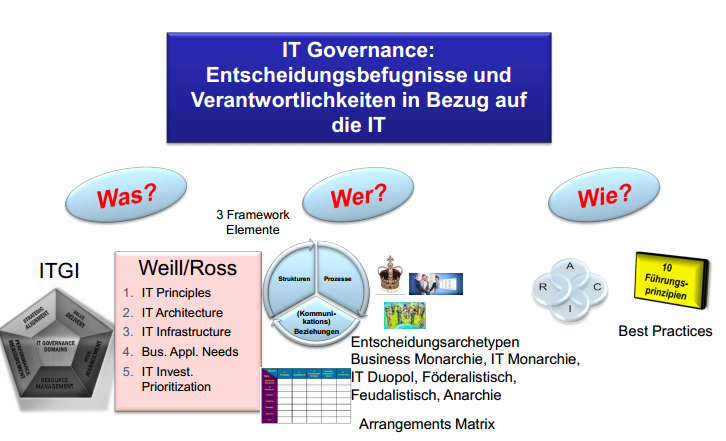
\includegraphics[width=0.8\linewidth]{fig/governance-big-picture}
\caption{IT Governance: Fasst alles zusammen, was man wissen muss.}
\label{fig:governance-big-picture}
\end{figure}

\section{Governance I}

\subsection{Begriff: IT Governance}
\textbf{Entscheidungsbefugnisse} und \textbf{Verantwortlichkeiten} in Bezug auf die IT.
\begin{quote}
	IT Governance specifies a framework for decision rights and accountability to encourage desirable behavior in the management and use of IT
\end{quote}


\subsection{Grundlegende Fragen zu Entscheidungen}
Diese Fragen, bzw. Elemente, müssen in einem Governance Rahmenwerk definiert werden.
\begin{description}
	\item[Was wird entschieden?] Governance Domains - Entscheidungsbereiche.
	\item[Wer entscheidet?] (Entscheidungsbefugniss)
	\item[Wie werden Entscheidungen umgesetzt?] Wie werden Entscheidungsfindungs-, ausführung und Verantwortlichkeiten implementiert.
\end{description}

\subsection{Differenzierung IT Management und IT Governance}
\paragraph{IT Management} Beschäftigt sich mit dem effizienten Betrieb der Unternehmens-IT. Software, Services, Infrastruktur, Projektdurchführung. Der Schwerpunkt liegt auf Administration Abläufe. Fokus auf interne Kunden. Stichwort \textbf{operativ}, Abteilungen und Individuen, Gegenwart, Kosten u. Qualität, Budgettreue, Durchführung.
\paragraph{IT Governance} Sichert, dass IT-Aktivitäten mit den aktuellen und zukünftigen Anforderungen des Business abgestimmt sind. Fokus auf interne und externe Kunden. Stichwort \textbf{strategisch}, Gesamtorganisation, Zukunft, Nutzen und Gewinn, sinnvolle Investitionen, Steuerung.

\subsection{Corporate Governance}
Umfasst die Strukturen und Prozesse zur Gesamtsteuerung des Unternehmens. Auf Ebene Verwaltungsrat und Geschäftsleitung. Im Mittelpunkt stehen Rechte und Interessen der Aktionäre und Teilhaber, Transparenz und Verantwortlichkeiten für die Entscheidungen.
Die Corporate Governance setzt somit Rahmen und Strukturen für die IT Governance.

\subsection{5 IT Governance Bereich (Domains) nach Weill/Ross}
\begin{description}
	\item[IT principles] Grundsätzliche Aussagen zum Stellenwert und zur Ausrichtung der IT. Basierend auf Geschäftsmodell. Welche Rolle spielt die IT? Entscheidender Wettbewerbsvorteil?
	\item[IT architecture] Regelt das Zusammenspiel zwischen Geschäftsarchitektur und IT Architektur. Stellt den Blueprint für die Integration, Entwicklung und Änderung der IT Assets zur Verfügung. Eine wohldefinierte, flexible EA ist eines der wichtigsten Governance Instrumente.
	\item[IT infrastruture] Strategie und Entscheide für die IT-Infrastruktur, die unternehmensübergreifend oder fachbereisübergreifend genutzt wird. Hardware, Software, IT Spezialisten. Angeboten als Services. Umfasst oft mehr als 50 Prozent der IT Kosten.
	\item[Business application needs] Wer definiert und genehmigt den Business Case. Definition der Projektverantwortung von den Requirements über Entwicklung zur Einführung. Wer entscheidet über die Architektur der Anwendung? EA-konform oder Innovationsausnahme?
	\item[IT investment prioritization] Wie viel und wo wird investiert? Durch welchen Prozess werden Projekte genehmigt? Wie erfolgt die Begründung eines Projekts? Projekt Portfolio Management?
\end{description}

\subsection{5 IT Governance Bereiche nach IT Governance Institute ITGI}
\begin{description}
	\item[Strategic alignment between Business and IT] Fortwährender Ausrichtung der IT an den Geschäftszielen und Geschäftsprozessanforderungen. Leistungen der IT in Art, Umfang und Qualität sind optimal auf die Bedürfnisse des Unternehmens ausgerichtet. Ziele für die IT sind klar definiert und von Businesszielen abgeleitet. Umsetzungsprozesse und –gremien exisitieren. IT Leistungen als Services verfügbar. Kontinuierliche Kommunikation zwischen Anbieter und Nutzer der IT Services. Investitionen klar am Unternehmensbedarf ausgerichtet.
	\item[Value delivery from IT to Business]. Wertbeitrag der IT ermitteln und stetig verbessern. Die IT von einer Unterstützungsfunktion zu einem Faktor der Wertschöpfung verändern. IT Dienstleistungen klar in Geschäftsprozesse integriert. Verwendung von Standards anstelle von proprietären	Individuallösungen. Überprüfung aller Prozessschritte und Aktivitäten auf Notwendigkeit und Wertbeitrag.
	\item[Management of the IT resources] Verantwortungsvoller und nachhaltiger Einsatz der Personal-, System- und Finanzressourcen. Ganzheitliche umfassende Betrachtung von Ressourcen und IT Prozessen. Prozesse sind standardisiert. Effiziente Gestaltung der IT Prozesse. Rollen und Verantwortlichkeiten sind klar definiert. Wissensmgmt. funktioniert.
	\item[Management of risks, security and rules] IT risiken identifizieren, richtig bewerten und angemessen behandeln. Risikotoleranz und Risikolevels sind für das Unternehmen definiert. Periodische Risikobewertung. Information Security Strategie existiert (abgenommen durch B. Hämmerli). Kosten proportional zum Wert eines IT Assets. 
	\item[Performance measurement] Transparenz der Leistungsstrukturen erhalten und Leistung messen und richtig beurteilen. Festlegung der Überwachung klar definierter Qualitätsmerkmale von IT Services. Regelmässiger Abgleich von Kennzahlen. Klar messbare Kennzahlen sind definiert.
\end{description}

\section{Governance II}
\subsection{Governance Entscheidungsarchetypen}
\subsubsection{Business Monarchie}
\textbf{Vorteile}
\begin{enumerate}
	\item Entscheidungen sind am Businessbedarf orientert
	\item Verantwortung des Business ist höher
	\item Schnelle Entscheidung
	\item Gute Umsetzungsunterstüzung vom Business
\end{enumerate}
\textbf{Nachteile}
\begin{enumerate}
	\item Zu wenig IT Knowhow
	\item Zu kurzfristig orientiert
	\item Zu kostenorientiert (zu wenig Investitionsbereit)
\end{enumerate}
\subsubsection{IT Monarchie}
\textbf{Vorteile}
\begin{enumerate}
	\item Technologisch gute Entscheidungen
	\item Auf IT Infrastruktur passende Lösungen
	\item Schnelle Trendserkennung
	\item Schnelle Entscheidung \& Umsetzung
\end{enumerate}
\textbf{Nachteile}
\begin{enumerate}
	\item Zu wenig kostenorientiert
	\item Technologieverliebte Entscheidungen, Einkauf unnötiger cooler Systeme
	\item Zu wenig Businessfokus, zu viel auf IT
\end{enumerate}
\subsubsection{Feudalistisch}
\textbf{Vorteile}
\begin{enumerate}
	\item Perfekt auf den Bereich zugeschnittene Lösungen
	\item Entscheidungen sind lokal verankert
	\item Schnelle Entscheidungen, da keine Abstimmung notwendig, keine Streitereien, jeder darf das haben was er haben will
	\item Hohe Dynamik
\end{enumerate}
\textbf{Nachteile}
\begin{enumerate}
	\item Heterogene Architektur
	\item Kostenintensive Integration
	\item Redundante Systeme
	\item Schlechter Informationsfluss
	\item Inseldenken
	\item Kaum übergreifende Lösungen -> IT Silos
	\item Kein Wissenstransfer
	\item KnowHow intensive IT
	\item Unternehmensweit unterschiedliches IT Wissen dass man nutzen muss
\end{enumerate}
\subsubsection{Föderalistisch}
\textbf{Vorteile}
\begin{enumerate}
	\item Breite Abstützung der Entscheidung
	\item Einheitliche Umsetzung ist einfacher
	\item Know How Transfer findet statt
	\item Hoher Meinungsaustausch, verschiedene Sichten, differenzierte Entscheidung möglich
\end{enumerate}
\textbf{Nachteile}
\begin{enumerate}
	\item Lange Entscheidungsprozesse
	\item Gefahr der Blockade einer Entscheidung - vorsichhenschieben der Entscheidung durch Grabenkämpfe, Krisen, gegenseitiges Blockieren...
	\item Teure Lösungen bei fehlenden Kompromissen
\end{enumerate}
\subsubsection{IT Duopol}
\textbf{Vorteile}
\begin{enumerate}
	\item Technisch und geschäftlich optimale Lösungen
	\item Transfer von Wissen zwischen Business \& IT
	\item Verbindung von Technologietrends \& Businessinnovation
	\item Gute Umsetzung
\end{enumerate}
\textbf{Nachteile}
\begin{enumerate}
	\item Verständnis \& Kommunikationsprobleme
	\item Gegenseitige Behinderung von Entscheidungen
\end{enumerate}
Unbedingt gemeinsame Ziele definieren!
\subsubsection{Anarchie}
\textbf{Vorteile}
\begin{enumerate}
	\item Sehr kurze Entscheidungsfristen (keine Absprachen nötig)
	\item Innovationsfreudig / Kreativ
\end{enumerate}
\textbf{Nachteile}
\begin{enumerate}
	\item Insellösungen / Adhoc Lösungen
	\item Heterogene IT Landschaften
	\item Hohe Wartungskosten
	\item Keine globale Strategie - grosse Investitionen sind nicht möglich
\end{enumerate}

\subsection{IT Governance Fallstricke}
\textbf{Symptome für Governance Probleme}
\begin{itemize}
	\item Bastellöusngen / SchattenIT
	\item Keine IT-Kennzahlen für Leistungsmessung / Bewertung de rIT
	\item Klagen über IT aus Management
	\item Redundante Systeme / Redundante Datenhalten
	\item IT entspricht nicht den Erwartungen
		\subitem Niedrige Kundenzufriedenheit
		\subitem Instabile Systeme
		\subitem Gescheiterte Projekte
	\item Explodierende IT Kosten bei niedrigem ROI
	\item IT Dienstleister nicht im Griff
\end{itemize}

\textbf{Massnahmen}
\begin{itemize}
	\item \textbf{Executive Engagement} \\
	IT Governance muss Chefsache werden
	\item \textbf{Policies as Strategic Tools} \\
		Es sollen klare und sinnvolle IT Prinzipien definiert werden, welche tatäschlich einen Nutzen bringen.
	\item \textbf{Defined Hierarchy of Governing Bodies} \\
		Wer was wie festlegen? Am besten eine Governence Arrangment Matrix aufbauen
	\item \textbf{Delegation of Authority and Precedent} \\
		Nicht zu viel zentralisieren bei den Entscheidungen, auch dezentrale Muster berücksichtigen.
	\item \textbf{Business Alignment} \\
		IT an Businessbedarf ausrichten
	\item \textbf{Proactive Liasion and Communications} \\
		Jeder Geschäftsbereich soll auf Management einen IT Ansprechspartner haben, der auch proaktiv auf sie zugeht und sie informiert.
	\item \textbf{Metrics and Reporting} \\
		Sinnvolle Kennzahlen definieren und erheben
	\item \textbf{Appropriate-Weight Procedures, Standards and Controls} \\
		Entscheidungen werden auf sinnvoller Ebene getroffen.
	\item \textbf{Independent Scrutiny} \\
		Das Reporting / Controlling wird von einer unabhängiger Instanz durchgeführt. Es geht nicht darum, die Leute zu überwachen, sondern um zu sehen ob es jetzt funktioniert.
	\item \textbf{Training and Awareness Program} \\
		Weiterbildung auf Governance Mechanismen
	\item \textbf{Easy-to-use Tools} \\
		Einfache Tools.
\end{itemize}